\chapter{Background}

\section{Recommendation Systems}
\subsection{Problem Statement}
Generally speaking, recommendation systems aim to support users in their decision making, while interacting with a large number of possible choices.
They recommend items to users based on their historical preferences.
Virtually, any decision making process can be made easier for users by providing recommendations.
Recommendation systems typically are used by online services, such as by Spotify for music~\cite{rec_spotify} and YouTube for videos~\cite{rec_yt}.
By using these online services, users generate data that the service can use to improve the recommendations.
To illustrate this point, rating videos indicates to the operator of the service how well the video is received by this specific user.
However, also retailers are known to use recommendation systems.
Based on data generated by customer loyalty programs such as Migros Cumulus~\cite{rec_migros}, retailers customize coupons or other offers to their customers.
In principle, it can be stated that data of users interacting with items (viewing, buying, rating etc.) constitute the basis for a recommendation system. 
Depending on the use-case, this data is utilized to assign scores to items depending on the user. 
The semantic meaning of a score depends on the objective of a recommendation system:
A system which recommends products to be bought might assign a "probability of purchase", whereas a system which recommends videos might predict the probability of a user watching a video to the end. 
\\
Bringing this all together we can define a general recommendation system with the following function:
\begin{equation}\label{eq:recommendation_system}
    s = f(i, u, h_u)
\end{equation}
Where $s$ is the assigned score to item $i$ for the user $u$ and the user's history $u_h$. 
The user's history represents all the previous interactions with items.
The aim of a recommendation engine is to determine the function $f$.
In order to assess the quality of the learned function, we need to establish the "true" score for the specific item and user, for which there are different ways.
During training, the learned functions are being tested on later interactions with items which are being held back.
Given the fact that as soon as the user sees the recommendation, his reality is changed, the performance of a recommendation engine in production also has to be assessed, i.e. the provider cannot be sure if or which recommendation in the user history led the user to the action.
\subsection{Properties of Recommendation Systems}
The following chapter gives a brief overview of different recommendation system properties.
Typically, recommendation systems consist of a combination of the following properties:
\paragraph{User-based}
User-based recommendation systems base their recommendations mainly on the properties of the user, such as gender or age, as well as the user's historical information, i.e. what he has bought or read before.
Thus, when generating recommendations for a specific user, the system tries to find similar users and recommends items those users liked.
\paragraph{Item-based}
Item-based recommendation systems use mostly information about the item to produce recommendations, such as item type (e.g. genre of a movie).
However, the basis for a recommendation is always a specific item, for example a product a user is looking at online.
The item the user is currently interacting with is referred to as the "active item". 
Usually, item-based recommendation systems then try to find similar items to the currently active item.
The method of finding similar items can be arbitrarily complex, which is why identifying similar items is its own field of research.
A common method is to combine this approach with a user-based component, where the similar items are sorted or filtered based on the user.
An example of this might be the following:
\begin{itemize}
    \item Steve is a male, looking at black shirts.
    \item When extracting similar products, we find a range of black shirts, including some women's shirts.
    \item If we would recommend items by popularity, the women's shirts would appear as the first recommendations, since women tend to buy more shirts.
    \item Instead of directly displaying the recommendations, we filter out the women's shirts that are part of this selection.
\end{itemize}
\paragraph{Session-based}
Session-based recommendation systems are a rather new form of such a system.
By definition, session is a sequence of interactions from a user with one or several items.
Depending on the use-case and setting, this can be defined differently.
Usually, online-services define a session as the sequence of interactions a user produces on the site until closing the browser window.
Based on this fact, session differ in length which is why it is difficult to directly feed that information into a recommendation system.
However, with the rise of recurrent neural networks (c.f.~\ref{rnn}) a powerful tool for handling variable length sequence data becomes available.
Session-based recommendation systems use RNNs to model the sequence data generated by sessions to achieve two things:
First, by using RNNs, a fixed dimensional representation of a specific session can be extracted, which allows the comparison of different sessions.
Second, by using the fixed representation of a session, the user's intent in a specific session can be identified and based on this, recommendations can be given in order to fulfill the user's intent.
An intent can be defined as the goal the user has in a specific session.
In the example of an online shop there are a few different, well-known intents identified by analysts such as: browsing for inspiration, searching for a specific product, buying a specific product, researching products.
Also these intents exist in different contexts, which in case of an online shop can be different product types (mobile phone, couch, dining table etc.).
The above mentioned explanation shows why these systems are more desired by operators of online services, as the recommendations can be targeted much more specifically to the user and his intent, instead of using just general information of the user and the active item. 
\paragraph{Collaborative}
Collaborative recommendation systems mostly use interaction data to generate recommendations.
Clicks on products are for example used as a data source in order to predict which products the user will click on next.
However, the collaborative aspect comes from the fact that we source other users' interactions as a basis for the recommendations.
In principle we interpret different users as versions of possible behavior of a user, the more interactions two users have in common, the more similar they are assumed to be.
Therefore, we can extend the behavior (i.e. product views) of a user by looking at what similar users have done on the same active item.
\paragraph{Content-based}
In contrast to collaborative recommendation systems, content-based systems heavily rely on so called content information.
Content information refers to the actual content of different items.
The name stems from early recommendation systems which mainly focussed on recommending media.
Given the assumption that a user likes to see items that are similar to each other (e.g. a user who mostly likes action films), the idea is to actually analyze the content of an item, be it the images in a movie, the soundwaves of a song or the text in a book.
However, this method can also be used in the context of online shopping, where the "content" of an item might be its textual description or an image of the actual product.
\subsection{Popular Examples}
In the following section, we will look at some popular examples of recommendation engines and their properties.
\subsubsection{Collaborative Filtering via Matrix Factorization}
As the name suggests, this model is a collaborative approach to a recommendation engine, meaning the model uses primarily interaction data between users and items.
As mentioned in~\cite{intro_recsys}, the main idea behind collaborative filtering is to recommend items to the user based on what users with similar taste liked in the past.
Collaborative filtering refers to a class of models that use similar users' tastes to recommend items.
Furthermore this class of models takes the user as a basis for recommendations, making it a user-based recommendation system.
As seen in~\cite{collaborative_filtering}, there are many ways of implementing a collaborative filtering system.
However, the essential part is the problem representation.

\begin{figure}[t]
	\centering
	\captionsetup{width=0.8\textwidth}
    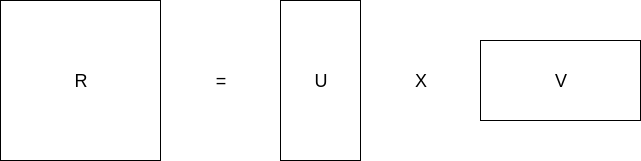
\includegraphics[width=\textwidth]{collaborative_filtering.png}
    \caption{Matrix Completion via Matrix Factorization}
    \label{fig:collaborative_filtering}
\end{figure}

In the Model-Based approach, the problem is represented as a matrix completion problem.
The matrix $R$ in figure~\ref{fig:collaborative_filtering} represents the interactions of users and items, where $r_{ij}$ represents the interaction of user $i$ with item $j$.
Usually, when dealing with such interaction data, this matrix is very sparse, since in general, a user interacts with a small set out of possibly millions of items.
The main idea behind this approach is to fill in the missing entries of the matrix.
In order to achieve this, two randomly randomly initialized matrices $U$ and $V$ are defined and when multiplied produce a matrix of the same shape as $U$.
As explained in~\cite{collaborative_filtering}, these two matrices represent low rank representations of users and items respectively.
The next step is to use an optimization algorithm to fit $U$ and $V$ such that $r_{ij} \approx (UV)_{ij}$.
The error of the chosen optimization algorithm however, is only applied to entries of $R$ which are known.
Therefore, when we find $U$ and $V$ such that the values for the known entries match the values in $R$, we assume that we also found a good approximation for the values unkown in $R$ and use these to predict the interaction of the respective users and items.

\subsubsection{Often Bought Together}\label{sec:often_bought_together}
Often bought together is a recommendation system very popular in online stores.
The idea behind it is to recommend products that complement the one the user is intending to buy.
A classical example for this would be to recommend a protection case when the users adds a smartphone to the basket, therefore it is an item-based approach.
The implementation of this recommendation system can be done in a rather simple way, but also be improved a lot by complex systems, which could personalize the recommendations by using the users history, and thereby extending it with a user-based component.
However, the basic idea remains to find items that are frequently bought together.
The simplest, yet still effective, implementation of this is to count the products appearing in the same order as other products, i.e. for each combination of two products $i$ and $j$, we will have a count $c_{ij}$ of how many times these products were bought together.
When a user adds a product to the basket, the products with the highest count are extracted from a database and recommended to users.

\section{Concepts}
\subsection{Recurrent Neural Networks}\label{rnn}
RNNs are a form of artificial neural networks, which allow to explicitly model sequence input data, because they allow the ouput of the network to be fed back in.
\begin{figure}[t]
	\centering
	\captionsetup{width=0.8\textwidth}
    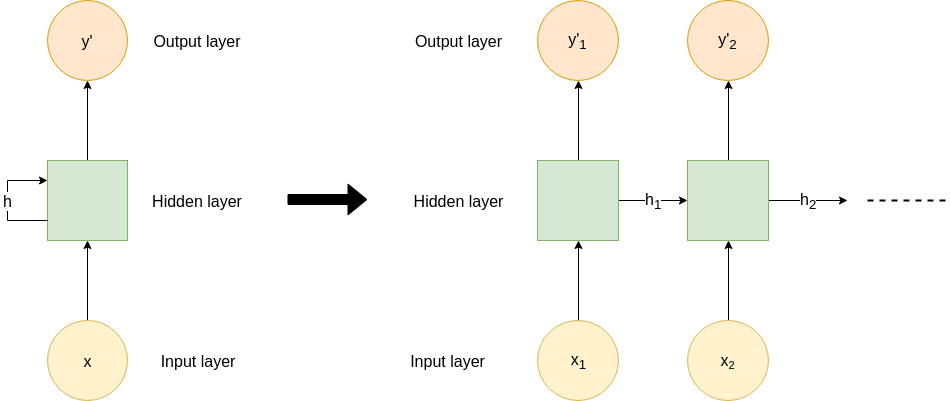
\includegraphics[width=\textwidth]{rnn.png}
    \caption{Recurrent Neural Network}
    \label{fig:rnn}
\end{figure}
Furthermore, RNNs carry a so called hidden state, which is propagated along the temporal axis.
The following two equations from~\cite{rnn_survey} describe the general behavior of a simple RNN unit as illustrated in figure~\ref{fig:rnn}.
\begin{equation}\label{eq:rnn_hidden_state}
    h_{i+1} = \sigma(W^{hx}x_i + W^{hh}h_i + b_h)
\end{equation}
\begin{equation}\label{eq:rnn_output}
    y'_i = \text{softmax}(W^{yh}h_i + b_y)
\end{equation}
We can see in equation~\ref{eq:rnn_hidden_state} how the hidden state is carried over.
This equation represents the connections across the temporal axis mentioned above.
Figure~\ref{fig:rnn} shows how the sequence input denoted by $x$ is unfolded and progressively fed into the network.
For each timestep, the corresponding output is computed as well as the hidden state that is carried over to the next timestep.
Intuitively, the hidden state can be seen as the variable holding the relevant information from the previous steps to influence the prediction of the next step.
\par
For clarification purposes, it is important to note that the individual inputs $x_t$ represent a datapoint in a sequence denoted by $x$, and therefore in most cases are represented by a vector.
In a feedforward neural network as illustrated in figure~\ref{fig:ffnn}, the inputs $x_i$ represent individual entries in the feature vector of the datapoint $x$.
\subsubsection{Backpropagation}
Backpropagation is the technique used to train neural networks.
\begin{figure}[t]
	\centering
	\captionsetup{width=0.8\textwidth}
    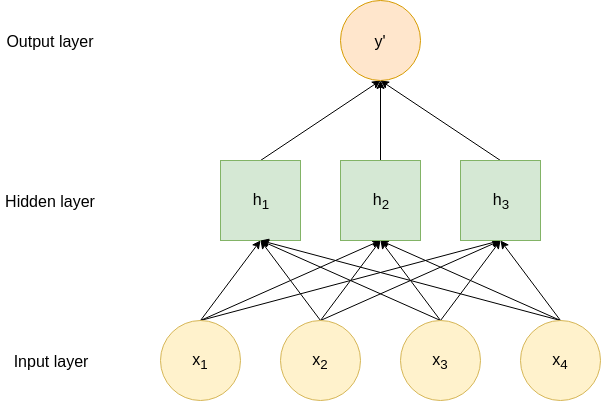
\includegraphics[width=0.8\textwidth]{ffnn.png}
    \caption{Feedforward Neural Network}
    \label{fig:ffnn}
\end{figure}
Let us assume we have a simple feedforward neural network as shown in figure~\ref{fig:ffnn}, the behavior of this network is described by the following equations.
\begin{equation}\label{eq:ffnn_hidden_layer}
    h_i = \sigma_h(w_{h_i}^Tx)
\end{equation}
\begin{equation}\label{eq:ffnn_output}
    y' = \sigma_y(w_{y}^Th)
\end{equation}
Each individual cell has a weight vector associated with it, denoted by $w_o$ where $o$ is the respective cell.
The arrows in the illustration represent the individual weights of such a weight vector.
Each layer has a nonlinear activation function associated with it, denoted by $\sigma_l$, $l$ being the respective layer.
\par
In this setting, we usually are in a supervised mode, where for each input $x$ there is a true label $y$.
Using the neural network we estimate $y$ for a given $x$ by applying the equations above to obtain the estimation $y'$.
\par
The last component needed before training is possible is a loss function $\mathcal{L}(y, y')$, which quantifies the error of the estimation $y'$.
\par
The basic idea of backpropagation is to attribute parts of the error computed to the different units of the network, and therefore make adjustements to the weight vector of a particular unit.
As described in~\cite{rnn_survey}, this is done by using the chain rule to compute the derivative of $\mathcal{L}(y, y')$ with respect to each weight vector.
The weight vector is then adjusted by gradient descent, i.e. by moving the vector in the direction of the largest decrease in the gradient.
Even though there are more parameters involved as for instance the learning rate, they are not essential for understanding the principle.
\subsubsection{Backpropagation with RNNs}
Also in~\cite{rnn_survey}, the authors mention that training RNNs has been known to be especially difficult due to the \emph{vanishing} or \emph{exploding gradients} problem.
Given the example of the RNN in figure~\ref{fig:rnn}, we compute the estimation $y'_t$, i.e. the output of timestep $t$.
As we can see in the equations~\ref{eq:rnn_hidden_state} and~\ref{eq:rnn_output}, this output is influenced by both, the current timestep and all the previous timesteps.
The problem now arises from the so called recurrent weights, denoted by $W^{hh}$, connecting the units across the temporal axis.
Assuming that the weights are small, i.e. $|w_{ij}| < 1$ for $w_{ij} \in W^{hh}$, the contribution of input $x_{t-k}$ to the output $y'_t$ gets exponentially smaller with increasing $k$.
By computing the gradient with respect to the input, the afromentioned contribution is quantified.
Therefore, when $k$ becomes large and the contribution of the input $x_{t-k}$ vanishes, the gradient with respect to the input unit vanishes as well, resulting in the so called vanishing gradient problem.
The opposite happens when the recurrent weights are large, i.e. $|w_{ij}| > 1$ for $w_{ij} \in W^{hh}$.
In this case, the contribution gets amplified when $k$ becomes large, which would lead to exploding gradients.
This represents problem in a setting where we want to learn long-range dependencies, which is often the case in sequence modeling.

\subsubsection{Gated Recurrent Unit}\label{sec:gru}
The Gated Recurrent Unit (GRU) is a recurrent unit which aims to solve the exploding or vanishing gradients problem mentioned above.
This is achieved by modifying the behavior of the hidden units, in between which the recurrent edges of the network are.
The authors of~\cite{gru} introduced this new type of recurrent unit.
They retrofitted the recurrent unit with the ability to adaptively remember and forget, by using the \emph{reset} and \emph{update} gate.
\par
The reset gate is responsible for supressing features of the hidden state that were learned to be unimportant for the future.
The reset gate is computed using the following formula:
\begin{equation}\label{eq:gru_reset_gate}
    r_t = \sigma( W_rx + U_rh_{t-1} + b_r)
\end{equation}
The matrices $W_r$ and $U_r$ as well as the bias $b_r$ are parameters specific to the reset gate and are learned simultaneously with backpropagation.
\par
The update gate controls how much information is propagated from the previous hidden state to the next one, i.e. it learns which features of the previous hidden state will be how important in the future.
The update gate is computed as follows:
\begin{equation}\label{eq:gru_update_gate}
    z_t = \sigma( W_zx + U_zh_{t-1} + b_z)
\end{equation}
Again, the weight matrices and bias are specific to the update gate and learned via backpropagation.
\par
To compute the next hidden state, the computed gates are used as follows:
\begin{equation}\label{eq:gru_hidden_state}
    h_t = z_t \circ h_{t-1} + (1 - z_t) \circ \text{tanh}(W_hx_t + U_h(r_t \circ h_{t-1}) + b_h)
\end{equation}
Equation~\ref{eq:gru_hidden_state} illustrates how the gates function.
When the reset gate is close to 0 in some features, the hidden state is forced to ignore that information before being multiplied with the weight matrix of the recurrent unit.
\par
On the other hand, the update gate controls how much information should be propagated directly from the hidden state, versus the hidden state resulting from the new input.
If the reset gate is 1 and the update gate is 0, we get the same formula as in~\ref{eq:rnn_hidden_state}, effectively returning to the vanilla RNN formulation.
\subsection{Embeddings of categorical variables}
A categorical variable is a variable that can take on one of a limited number of values.
Examples are colors, locations or, in the context of e-commerce, product IDs.
When using such variables as an input variable for some model, the variables need to be transformed into a numerical representation, allowing the variable to be used.
Assuming that we have a variable which describes the color of a specific product -- for reasons of simplicity with only the four colors red, green, blue, and yellow -- one possibility would be to just integer IDs to the different colors as shown in table~\ref{tab:id_encoding}.
\begin{table}[t]
    \centering
    \begin{tabular}{ll}\toprule
    \textbf{Color} & \textbf{ID} \\ \midrule
    Red & 0 \\
    Green & 1 \\
    Blue & 2 \\
    Yellow & 3 \\ \bottomrule
    \end{tabular}
    \caption{Integer IDs for Colors}
    \label{tab:id_encoding}
\end{table}
This approach entails the problem that integers have a defined order.
That means that any model will interpret the color yellow as larger or as a stronger signal, than the color red.
This is not desirable, in the case of colors, all of them should have the same magnitude.
\par
A different way of representing categorical variables is the so called one-hot encoding.
A one-hot encoding requires a continuous ID space, such as the one in table~\ref{tab:id_encoding}.
The same colors encoded in a one-hot encoding can be seen in table~\ref{tab:one_hot_encoding}.
\begin{table}[t]
    \centering
    \begin{tabular}{ll}\toprule
        \textbf{Color} & \textbf{One-Hot Encoding} \\ \midrule
    Red & $[1,0,0,0]$ \\
    Green & $[0,1,0,0]$ \\
    Blue & $[0,0,1,0]$ \\
    Yellow & $[0,0,0,1]$ \\ \bottomrule
    \end{tabular}
    \caption{One-Hot Encoding for Colors}
    \label{tab:one_hot_encoding}
\end{table}
This ensures all the color representations have the same magnitude, therefore the model will get the same signal strength from each of the colors.
We basically transform the id encoding to a one-hot encoding by using a zero vector of dimension $\max(\text{ID})$ and set the element at the position $\text{ID}_x-1$ to 1, for item $x$.
Therefore, the one-hot encoding always has the same dimensionality as the number of categories.
There are still two major drawbacks to this approach.
As we will see in section~\ref{sec:dataset_properties}, the number of categories for such a variable can reach into the millions.
This means that the dimensionality of the single categorical feature can range into the millions.
This is not desirable, since high dimensionality leads to more difficulties in training and more computing resources needed to accomplish the training task.
The second drawback is that this representation does not account for the notion of similarity, i.e. red is as similar to blue as it is to yellow.
However, it is known that green is a composition of blue and yellow, so green should be more similar to blue and yellow than to red.
\par
These two issues can be solved by using embeddings.
Embeddings are a low dimensional real numbered representation of a categorical variable; similar variables will have similar vectors representing them.
The difficulty with embeddings is finding a process which produces the embeddings with the desired properties.
For a small number of variables it is possible to manually construct them.
In table~\ref{tab:embedding}, we can see a lower dimensional representation of the same colors, however, the distance between green and yellow or blue is smaller than the one between green and red.
As all the representations still have the same magnitude none of the colors triggers a stronger signal.
\begin{table}[t]
    \centering
    \begin{tabular}{ll}\toprule
    
    \textbf{Color} & \textbf{Embedding} \\ \midrule
    Red & $[1,0,0]$ \\
    Green & $[0,\sqrt{0.5},\sqrt{0.5}]$ \\
    Blue & $[0,1,0]$ \\
    Yellow & $[0,0,1]$ \\ \bottomrule
    \end{tabular}
    \caption{Possible Embedding for Colors}
    \label{tab:embedding}
\end{table}

\section{Previous Work}
\subsection{Meta-Prod2Vec}\label{sec:meta_prod2vec}
Meta-Prod2Vec is a method proposed in~\cite{meta_prod2vec} to compute such embeddings as described in the previous section.
The original inspiration for this approach comes from the famous \emph{word2vec} model (c.f.~\cite{word2vec}), a method of computing embeddings for words, respecting the similarity between them.
Based on word2vec, Yahoo developed a model named \emph{prod2vec} (c.f.~\cite{prod2vec}), that computes embeddings of products using the receipts their customers are receiving in their inbox.
Meta-Prod2Vec is an extension of prod2vec that allows to include meta information about products, such as brands and product type.
\par
The fundamental assumption behind all of the afromentioned models is the famous Distributional Hypothesis~\cite{distributional}, which states that words appearing in the same context have similar, if not identical, meaning.
For illustration purposes consider the following two example sentences:
\begin{itemize}
    \item George likes to drink a glass of wine in the evening.
    \item George likes to drink a glass of whiskey in the evening.
\end{itemize}
Without knowing the meaning of the words "wine" or "whiskey", one could deduce that they are at least similar concepts.
Essentially, the context of a word limits the number of possible words that can appear in that context.
If that context is restrictive enough, there are only few possible words or concepts that can occur in that context.
This assumption is translated into the context of e-commerce by interpreting products as words and sessions or purchase sequences as sentences.
\par
Since Meta-Prod2Vec is an extension of prod2vec, it makes sense to first look at the loss function of prod2vec in equation~\ref{eq:prod2vec_loss}:
\begin{equation}\label{eq:prod2vec_loss}
    L_{J|I} = \sum_i X_iH(p_{\cdot|i},q_{\cdot|i})
\end{equation}
Where $X_i$ is the number of occurences of word $i$ and $H(\cdot)$ is the cross entropy loss.
$J$ describes the output space, whereas $I$ is the input space, in this context they are the same, specifically all the possible products.
The loss function is the weighted cross entropy loss between the empirical probability distribution $p_{\cdot|i}$ and the predicted probability distribution $q_{\cdot|i}$.
The weighted cross entropy loss forces the predicted probability for any product to be close to the observed empirical probability.
This means that the learned probability function $q_{\cdot|i}$, in the case of observed events, is close to to the empirical probability distribution, while also allowing predictions of yet unseen events.
\par
In the next step, we look at the learned probability function $q_{\cdot|i}$, and how it is related to the embeddings of products.
In equation~\ref{eq:prod2vec_softmax} we can see how $q_{\cdot|i}$ is defined:
\begin{equation}\label{eq:prod2vec_softmax}
    q_{j|i} = \frac{\exp(w_i^Tw_j)}{\sum_{j \in V_J} \exp(w_i^Tw_{j})}
\end{equation}
This defines the probability that product $j$ is in the context of product $i$.
In principle this means, that the inner product $w_i^Tw_j$ is interpreted as an unnormalized probability, and by applying the softmax function, we obtain a probability distribution over all possible context words $V_J$.
\par
From looking at the two equations above, it is apparent that computing this loss function is rather expensive, the complexity is $O(n^2)$ for $n$ being the number of products.
Therefore, these models are usually trained using negative sampling loss~\cite{neg_sampling}.
\par
The loss function of Meta-Prod2Vec, as seen in equation~\ref{eq:meta_prod2vec_loss} is a natural extension of the loss function of prod2vec.
\begin{equation}\label{eq:meta_prod2vec_loss}
    L_{MP2V} = L_{J|I} + \lambda \cdot (L_{M|I} + L_{J|M} + L_{M|M} + L_{I|M})
\end{equation}
Where $\lambda$ is a regularization parameter controlling how much the side information influences the total loss and $M$ describes the metadata space.
In the following, the different components of the loss function are presented:
\begin{itemize}
    \item $L_{J|I}$: This is the same term as in equation~\ref{eq:prod2vec_loss}, it describes the cross entropy between the observed conditional probability and the modeled conditional probability of the output products conditioned on the input products.
    \item $L_{M|I}$: This is the loss component of the probability distribution of metadata values of surrounding products, given the input product.
    \item $L_{J|M}$: This component measures the loss of the probability distribution of surrounding products, given the metadata values of the input product.
    \item $L_{M|M}$: This is the loss incurred from the probability distribution of surrounding products metadata, given the metadata values of the input product.
    \item $L_{I|M}$: Finally this component measures the loss of the probability distribution of the input products, given their own metadata values.
\end{itemize}
In principle, the objective function in equation~\ref{eq:prod2vec_loss} is extended to include all possible interaction terms with the metadata.
The advantage of this loss function is that it does not change the training algorithm of prod2vec.
The only thing changing is the data generation process; additionally to creating the pairs of co-occurring products, also co-occurring metadata and products are generated.
Since the individual components of the loss function are computed in exactly the same way, adding these co-occurence terms will automatically compute the total loss.
Thus, the metadata values will be embedded in the same output space.
\subsection{Personalized Session-based Hierarchical Recurrent Neural Network}\label{sec:hgru4rec}
The work presented in~\cite{hierarchical} serves as a basis for this thesis.
The authors present a model architecture that can model the session behavior of users, as well as learn historical user preferences and apply those to the recommendations.
This makes it a user- and session-based recommendation system.
The architecture presented is based on a model called \emph{gru4rec} presented in~\cite{gru4rec}.
In figure~\ref{fig:hgru4rec}, we can see an illustration of the model architecture.
Essentially, the difference between gru4rec and hgru4rec is the addition of the the second level GRU, $GRU_{u}$, which keeps track of historical user preferences.
\begin{figure}[t]
	\centering
	\captionsetup{width=0.8\textwidth}
    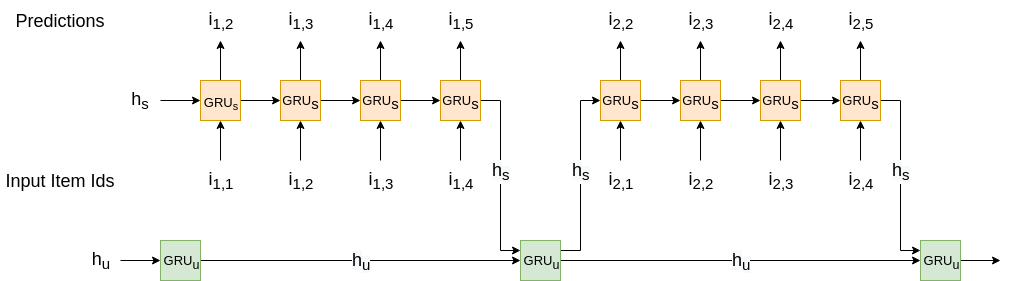
\includegraphics[width=\textwidth]{hgru4rec.png}
    \caption{hgru4rec model architecture}
    \label{fig:hgru4rec}
\end{figure}
To formalize the sessions of users, we define the sessions of a specific user $u$ as $\mathcal{S}_u = \lbrace s_u^1, s_u^2, \cdots, s_u^n \rbrace $.
A session is defined as $s_u^k = \lbrace e^k_1, e^k_2, \cdots, e^k_m \rbrace $, where an event $e^k_n$ is the product id of the product viewed in session $k$ at position $n$.
\par
The proposed model uses the session level GRU, $GRU_s$, to predict the next item that the user would view.
The hidden state $h_s$ serves as a fixed size representation of the session.
The input to the GRU is defined as follows: $i_{m,n} = \text{onehot} ( e^m_n )$, where $\text{onehot}(x)$ is the one-hot encoding of the integer $x$.
Now the output and the next hidden state are computed, using the formula introduced in~\ref{sec:gru} as follows:
\begin{equation}\label{eq:hgru4rec_session}
    r_{m,t}, h_m^{t} = GRU_s(i_{m,n-1}, h_s^{t-1})
\end{equation}
Where $h_m^{t}$ is the session hidden state of session $m$ at time $t$ and $r_{m,t}$ is a score for every item to be recommended in session $m$ at time $t$.
The output of the GRU, $r_{m,t}$, is compared to the one-hot encoding of the next item, i.e. $i_{m,t+1}$ to compute the loss function.
The loss function was explicitly designed by the authors for this task.
The TOP1 loss is the regularized approximate relative rank of the relevant item.
The relative rank of the relevant item in the next step is defined in equation~\ref{eq:relative_rank}:
\begin{equation}\label{eq:relative_rank}
    \text{relative rank} = \frac{1}{N}\cdot \sum_{j=1}^{N} I\lbrace r_{m,t}^j > r_{m,t}^i \rbrace
\end{equation}
Where $N$ is the number of items, $r_{m,t}^k$ is the score of item $k$ in session $m$ at time $t$ and finally $i$ is the relevant item in the next step.
This function computes the number of items which have a higher score than the relevant item.
However, this relative rank has two drawbacks: First, the indicator function is difficult to derive and second, the computation of the loss for one item involves the computation of the score for all possible items.
Therefore, the relative rank is approximated by the equation~\ref{eq:top1_loss}, which further includes a regularization term forcing the irrelevant item scores towards zero.
\begin{equation}\label{eq:top1_loss}
    L_{TOP1} = \frac{1}{N_S} \cdot \sum_{j=1}^{N_S} \sigma(r_{m,n}^j - r_{m,n}^i) + \sigma(r_{m,n}^j)
\end{equation}
Where $N_S$ is the number of sampled irrelevant items to avoid the computation of the scores for every item and $\sigma$ is a sigmoid function.
The sampling method will be described in more detail, when presenting at the dataset (c.f.~\ref{sec:dataset}).
This loss function includes an additional regularization term, which should motivate the scores of the sampled irrelevant items to be close to 0.
\par
After a session is completed, the user-level GRU, $GRU_u$, comes into play.
The task of this GRU is to learn how the session representation of users change over time.
This is achieved by using the fixed size session representation as the input to $GRU_u$.
The output of $GRU_u$ then will serve as the new initial session hidden state for the next session.
\begin{equation}\label{eq:hgru4rec_user}
    h_u^m, h_m^0 = GRU_u(h_u^{m-1}, h_{m-1}^{n_{m-1}})
\end{equation}
Where $h_u^m$ is the hidden state of user $u$ at the beginning of session $m$ and $n_m$ is the number of items in session $m$.
\par
Both GRUs are trained jointly using the same loss function.

\section{Key Performance Indicators}
Key Performance Indicators (KPIs) are metrics used in a business process to measure the performance of said process.
In online services there are a few well established metrics; most relevant for this work are the click-through rate and the conversion rate.
These metrics are also often used in testing multiple versions of the same element, for example a new design of a button.
By measuring these metrics, it can be determined which version most users prefer.
\paragraph{Click-Through Rate}
The click-through rate (CTR) measures how many users click on a specific element relative to the number of impressions.
Impressions are defined as the event when a user has the specific element that is measured in his viewport.
Finally, the viewport is the part of the website or web application which is visible to the user in his browser window.
In equation~\ref{eq:ctr}, its formalization is shown.
\begin{equation}\label{eq:ctr}
    \text{CTR} = \frac{\#\text{clicks}}{\#\text{impressions}}
\end{equation}
\paragraph{Conversion Rate}\label{sec:conversion_rate}
The conversion rate measures how many successful transactions follow the interaction with a specific element.
A transaction can be defined in a rather abstract way, such as listening to a song, or watching a video to the end.
In the context of e-commerce however, the conversion rate measures how many successful sales are made following an interaction with an element.
This is formalized in equation~\ref{eq:conversion_rate}.
\begin{equation}\label{eq:conversion_rate}
    \text{Conversion Rate} = \frac{\#\text{sales}}{\#\text{impressions}}
\end{equation}
Since there might be multiple elements for which the conversion rate is measured, there needs to be a strategy of attributing sales to specific elements in the web application.
An exact way of computing the conversion rate is therefore difficult to find, but there are multiple ways to approximate this value.
One common way is if the user sees an impression of a specific element and completes a purchase in the same session, then this element receives credit for the sale.
This approach entails the problem that the user is not tracked across multiple sessions.
The session in which the user finds this item, and the session in which the user actually makes the purchase are often not the same.
Also, if the user receives an impression, it is not clear whether the user actually registers the item, or if the user is focused on another part of the application.
Finally, this method credits sales to an element even if the purchased product was not even recommended.
Thus, we chose another approximation of this metric.
If a user purchases an item that was recommended and then clicked by the user, and the click is less than 14 days before the purchase, the element receives credit for the sale.
The number 14 days was chosen because more than 99\% of product sales, which were clicked by the users after being recommended, fall into this range.